\problemname{Pipe Rotation}


\noindent The four ninja turtles:  Leonardo, Donatello, Michelangelo, and Raphael 
are seeking a new home in Manhatten, New York City. The turtles don't like sudden deadends 
in their home. Fortunately the government recently installed a new sewage system where pipes 
can be rotated! The turtles needs your help finding a suitable home so they're willing to provide you a grid 
describing the current layout of the sewage system.  \\

\noindent The grid consists of R and C columns. The cell $G_{r,c}$ will be one of 4 pipes encoded as a 
between "A" and "D". These pipes can be rotated by any multiple 
of 90 degrees: \\

\begin{minipage}{0.4\textwidth}
  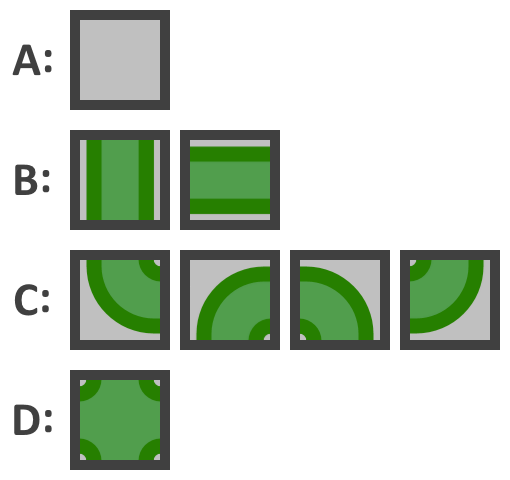
\includegraphics[width=.7\textwidth]{pipe_rotation_1.png} 
\end{minipage} \hfill
\begin{minipage}{0.6\textwidth}
  \begin{itemize}
    \item (A) Nothing
    \item (B) Straight pipe (pipes leaving through 2 opposite edges)
    \item (C) Elbow-shaped pipe (pipes leaving through 2 adjacent edges)
    \item (D) Four-way pipe (pipes leaving through all 4 edges) 
  \end{itemize}
\end{minipage} 
\\ 


\noindent Determine whether or not it's possible to rotate the cells such that the pipes all 
line up with one another. In particular, for each edge shared by a pair of adjacent cells, 
there must either be a pipe on both sides of that edge, or on neither side. 
And for each each of the $2 \cdot (R+C)$ outer edges of the grid, there must be no pipe leaving through that edge. Below are examples:


\begin{figure}[h]
  \centering
  \begin{minipage}[t]{0.45\textwidth}\centering%
      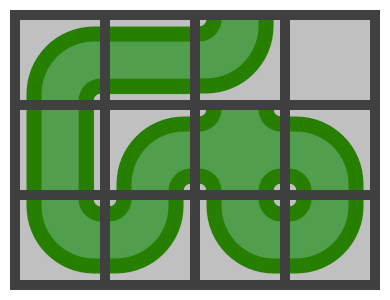
\includegraphics[width=\textwidth]{pipe_rotation_2}
      \caption{invalid example, two sudden deadends}
  \end{minipage} \hfill
  \begin{minipage}[t]{0.45\textwidth}\centering%
      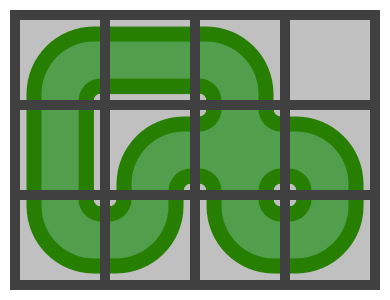
\includegraphics[width=\textwidth]{pipe_rotation_3} 
      \caption{valid example, no sudden deadends}
  \end{minipage}
\end{figure}

% \begin{minipage}{0.4\textwidth}
%   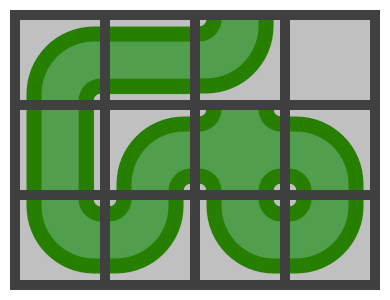
\includegraphics[width=\linewidth]{pipe_rotation_2.png} \hfill
%   \caption{example invalid example}
% \end{minipage} \hfill
% 
% \begin{minipage}{0.4\textwidth}
%   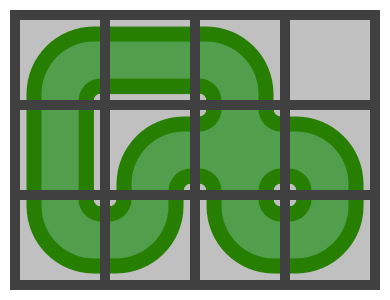
\includegraphics[width=\linewidth]{pipe_rotation_3.png}
%   \caption{example valid image}
% \end{minipage}

% \begin{figure}[h]
%   \minipage{0.32\textwidth}
%   \endminipage\hfill
%   \minipage{0.32\textwidth}
%   \endminipage\hfill
%   \minipage{0.32\textwidth}%
%     \caption{A really Awesome Image}\label{fig:awesome_image3}
%   \endminipage
% \end{figure}




\section*{Input}
Line 1: 2 integers, R and C \\
Next R lines: C characters, $G_{i,1..C}$, for i=$1..R$ \\

\section*{Output}
A string, either "Possible" if it's possible to produce a valid grid, or "Impossible" otherwise
